\documentclass[a4paper, twocolumn]{ltjsarticle}
\usepackage[top=25mm, bottom=25mm, left=20mm, right=20mm]{geometry}

% 画像
\usepackage[dvipdfmx]{graphicx}
\usepackage{ascmac}
\usepackage{array}
% 表
\usepackage{booktabs}
\usepackage{enumerate}

% 数式
\usepackage{amsmath}
\usepackage{amssymb}
\usepackage{amsfonts}
\usepackage{float}

% ベクトル
\usepackage{bm}
% コード
\usepackage{listings,jvlisting}
% コードの色
\usepackage{color}
\definecolor{OliveGreen}{rgb}{0.0,0.6,0.0}
\definecolor{Orenge}{rgb}{0.89,0.55,0}
\definecolor{SkyBlue}{rgb}{0.28,0.28,0.95}
% ここからコードの表示に関する設定
\lstset{
  basicstyle={\ttfamily},
  identifierstyle={\small},
  commentstyle={\small\itshape},
  keywordstyle={\small\bfseries},
  ndkeywordstyle={\small},
  stringstyle={\small\ttfamily},
  frame= single,
  breaklines=true,
  columns=[l]{fullflexible},
  numbers=none,
  xrightmargin=0.3cm,
  xleftmargin=0.2cm,
  numberstyle={\scriptsize},
  stepnumber=1,
  keepspaces=true,
  keywordstyle={\color{SkyBlue}},
  commentstyle={\color{OliveGreen}},
  stringstyle=\color{Orenge},
  showstringspaces=false
}
\renewcommand{\lstlistingname}{Code}
\newcommand{\E}[1]{\times10^{#1}}
\usepackage{caption}
\usepackage{subcaption}

\title{人工知能 期末レポート 課題12}
\author{03420414  小松麟太郎}
\date{\today}


\begin{document}

\maketitle

\section{序論}
本課題では，メタヒューリスティックスを用いた多目的最適化シミュレーターを作成した．MOABC（Multi-Objective Artificial Bee Colony）とMOGWO（Multi-Objective Gray Wolf Optimization）の2つのアルゴリズムを実装し，2つの関数に対してどちらかのアルゴリズムを選択して最適化を行うことができるようにした．本レポートでは，2つのアルゴリズムの概要，シミュレーターの使用方法，及び性能評価について述べる．

\section{アルゴリズム}
本章ではシミュレーターに用いたMOABCとMOGWOの2つのアルゴリズムについてそれぞれ説明する．
\subsection{外部アーカイブ}
メタヒューリスティクスを用いた多目的最適化アルゴリズムでは，探索によって得られた非劣解を集団内に保持することが困難である．そこで，集団とは別に外部アーカイブ（External Archive，EA） を用意し，探索中に得られた非劣解を記録・管理する．外部アーカイブを活用することで，過去の優れた解を保持しつつ，多様性を維持しながら最適化を進めることが可能となる．本課題で用いた MOABCと MOGWOも外部アーカイブを採用している．\\\quad
外部アーカイブは，世代が1つ進むごとに更新される．新たに得られた解が既存の解よりも優れている場合，既存の解を外部アーカイブから削除し，新しい解を追加する．この更新を繰り返すことで，外部アーカイブには次第に非劣解が蓄積されていく．しかし，外部アーカイブのサイズが無制限では，計算コストが増大し，最適化の効率が低下する．そのため，外部アーカイブのサイズを一定数に制限し，新たな解を追加する際には，既存の解の一部を削除する必要がある．\\\quad
外部アーカイブから解を削除する際には，多様性を維持するための戦略が求められる．本課題では，混雑距離（Crowding Distance）を指標として解の選択を行う．混雑距離とは，外部アーカイブ内の各解について，最近傍の解との目的関数値の差を総和したものである．この値が大きいほど，その解の周囲には比較的多くの解が存在することを示す．そのため，混雑距離が大きい解から順に削除することで，非劣解の分布を均等に保ち，多様性を確保することができる．
\subsection{MOABC}
MOABC[1]は，ABC（Artificial Bee Colony）を多目的最適化に拡張したアルゴリズムである．元のABCでは蜂の群れをEmployed Bee，Onlooker Bee，Scout Beeの3つのグループに分け，それぞれの蜂が探索を行うことで最適解を探索するが，MOABCでは全ての蜂をOnlooker Beeとして扱い，外部アーカイブを蜜源として探索する．\\\quad
Onlooker Bee の個体数を $N$，$i$ 番目の個体のいる蜜源（関数の入力ベクトル）を $\boldsymbol{x}_i$ とする．まず，$\boldsymbol{x}_i$ をランダムに初期化し，そのうち非劣解を外部アーカイブに保存する．蜜源の更新は次のように行われる．まず，外部アーカイブからランダムに2つの要素 $\boldsymbol{e}_k$ と $\boldsymbol{e}_l$ を蜜源として選択する．そして，$\boldsymbol{x}_i$ の中からランダムに $m$ 次元を選び，$m$ 次元は $\boldsymbol{e}_k$，その他の次元は $\boldsymbol{e}_l$ をもとに新たに $\boldsymbol{v}_i$ を生成する．$j$ 番目の次元における $\boldsymbol{v}_i$ の値 $v_{ij}$ は以下のように計算される．
\begin{equation}
    v_{ij} = 
    \begin{cases}
        x_{ij} + \mathrm{rand}(0, 2)(e_{kj} - x_{ij}) &\\
        x_{ij} + \mathrm{rand}(0, 2)(e_{lj} - x_{ij}) &
    \end{cases}
\end{equation}
ここで，$\mathrm{rand}(a, b)$ は区間 $[a, b]$ の一様乱数を生成する関数である．$\boldsymbol{v}_i$ が $\boldsymbol{x}_i$ よりも優越している場合，Onlooker Beeは $\boldsymbol{x}_i$ から $\boldsymbol{v}_i$ に移動し，$\boldsymbol{v}_i$ を外部アーカイブに保存する．元の $\boldsymbol{x}_i$ が $\boldsymbol{v}_i$ よりも優越している場合は何もしない．そして，互いに優越していない場合は，$\boldsymbol{v}_i$ を外部アーカイブに保存し，Onlooker Beeは1/2の確率で $\boldsymbol{v}_i$ に移動する．最後に2.1節で述べた方法に従って，外部アーカイブの更新を行う．MOABCのアルゴリズムの疑似コードは以下のようになる．

\begin{lstlisting}
世代数 = 1
蜜源 x_i (i = 1,...,N) をランダムに初期化
各蜜源の関数値を計算
非劣解を外部アーカイブ(EA)に保存
while 世代数 < 最大世代数 do
    for each Onlooker Bee do
        EA からランダムにベクトルを選択
        式(1)からベクトル v_i を生成
        v_iの関数値を計算
        EAとx_iを更新
    end for
    非劣解のみをEAに保持
    if EA のサイズが上限を超えた
        混雑距離を用いて解を削除
    end if
    世代数 = 世代数 + 1
end while
\end{lstlisting}    
\subsection{MOGWO}
MOGWO[2]は，GWO（Gray Wolf Optimization）を多目的最適化に拡張したアルゴリズムである．GWOはGray Wolfの群れの中から，アルファ，ベータ，デルタの3つの優秀な個体を選び，それぞれの位置をもとにして他の個体が探索を行うことで最適解を探索する．MOGWOでは，外部アーカイブから，混雑距離の逆数で重みづけした確率に従って，アルファ，ベータ，デルタを選択する．こうすることによって，周囲にほかの個体が比較的少ない個体を選択することができ，多様性を保つことができる．群れの個体数を $N$，$i$ 番目の個体のいる位置（関数の入力ベクトル）を $\boldsymbol{x}_i$，アルファ，ベータ，デルタをそれぞれ $\boldsymbol{e}_\alpha$，$\boldsymbol{e}_\beta$，$\boldsymbol{e}_\delta$ として，$\boldsymbol{x}_i$ を次の手順で更新する．まず，次のようにベクトル $\boldsymbol{a}_i$，$\boldsymbol{c}_i$，$(i = 1, 2, 3)$ を生成する．
\begin{align}
    \boldsymbol{a}_i &= 2\boldsymbol{r}_i\odot\boldsymbol{a'}-\boldsymbol{r}_i\\
    \boldsymbol{c}_i &= 2\boldsymbol{r'}_i
\end{align}
ここで，$\boldsymbol{r}_i$，$\boldsymbol{r'}_i$ は区間 $[0, 1]$ の一様乱数を要素に持つベクトル．$\boldsymbol{a'}$ は世代が進むにしたがって各要素が2から0まで線形に減少するベクトルである．$\odot$ はアダマール積であり，要素ごとの積を表す．そして，$\boldsymbol{a}_i$，$\boldsymbol{c}_i$ を用いて，$\boldsymbol{x}_i$ から $\boldsymbol{v}_i$ を計算する．
\begin{align}
    \boldsymbol{d}_\alpha &= |\boldsymbol{c}_1\odot\boldsymbol{e}_\alpha-\boldsymbol{x}_i|\nonumber\\
    \boldsymbol{d}_\beta &= |\boldsymbol{c}_2\odot\boldsymbol{e}_\beta-\boldsymbol{x}_i|\\
    \boldsymbol{d}_\delta &= |\boldsymbol{c}_3\odot\boldsymbol{e}_\delta-\boldsymbol{x}_i|\nonumber
\end{align}
\begin{align}
    \boldsymbol{x}_\alpha &= \boldsymbol{e}_\alpha-\boldsymbol{a}_1\odot\boldsymbol{d}_\alpha\nonumber\\
    \boldsymbol{x}_\beta &= \boldsymbol{e}_\beta-\boldsymbol{a}_2\odot\boldsymbol{d}_\beta\\
    \boldsymbol{x}_\delta &= \boldsymbol{e}_\delta-\boldsymbol{a}_3\odot\boldsymbol{d}_\delta\nonumber
\end{align}
\begin{align}
    \boldsymbol{v}_i &= \frac{\boldsymbol{x}_\alpha+\boldsymbol{x}_\beta+\boldsymbol{x}_\delta}{3}
\end{align}
ここで，$\boldsymbol{d}$もベクトルであり，式(4)の絶対値は，各要素ごとに計算される．この$\boldsymbol{v}_i$ を Gray Wolf の次世代の位置として更新する．$\boldsymbol{v}_i$ が外部アーカイブの非劣解である場合，$\boldsymbol{v}_i$ を外部アーカイブに保存する．最後に2.1節で述べた方法に従って，外部アーカイブの更新を行う．MOGWOのアルゴリズムの疑似コードは以下のようになる．
\begin{lstlisting}
世代数 = 1
Gray Wolfの位置 x_i (i = 1,...,N) を初期化
各x_iの関数値を計算
非劣解を外部アーカイブ(EA)に保存
while 世代数 < 最大世代数 do
    for each Gray Wolf do
        EA からアルファ，ベータ，デルタを選択
        式(2)-(6)からベクトル v_i を生成
        v_iの関数値を計算
        EAとx_iを更新
    end for
    非劣解のみをEAに保持
    if EA のサイズが上限を超えた
        混雑距離を用いて解を削除
    end if
    世代数 = 世代数 + 1
end while
\end{lstlisting}
\section{使用方法}
本章では作成したシミュレーターの使用方法について説明する．シミュレーターは python で実装されており，GUIはcustomtkinterを用いて作成した．実行にはcustomtkinterとtkinterが必要である．インストールされていない場合は，以下のコマンドでインストールする．
\begin{lstlisting}
$ pip install tk
$ pip install customtkinter
\end{lstlisting}
\begin{figure}[t]
    \centering
    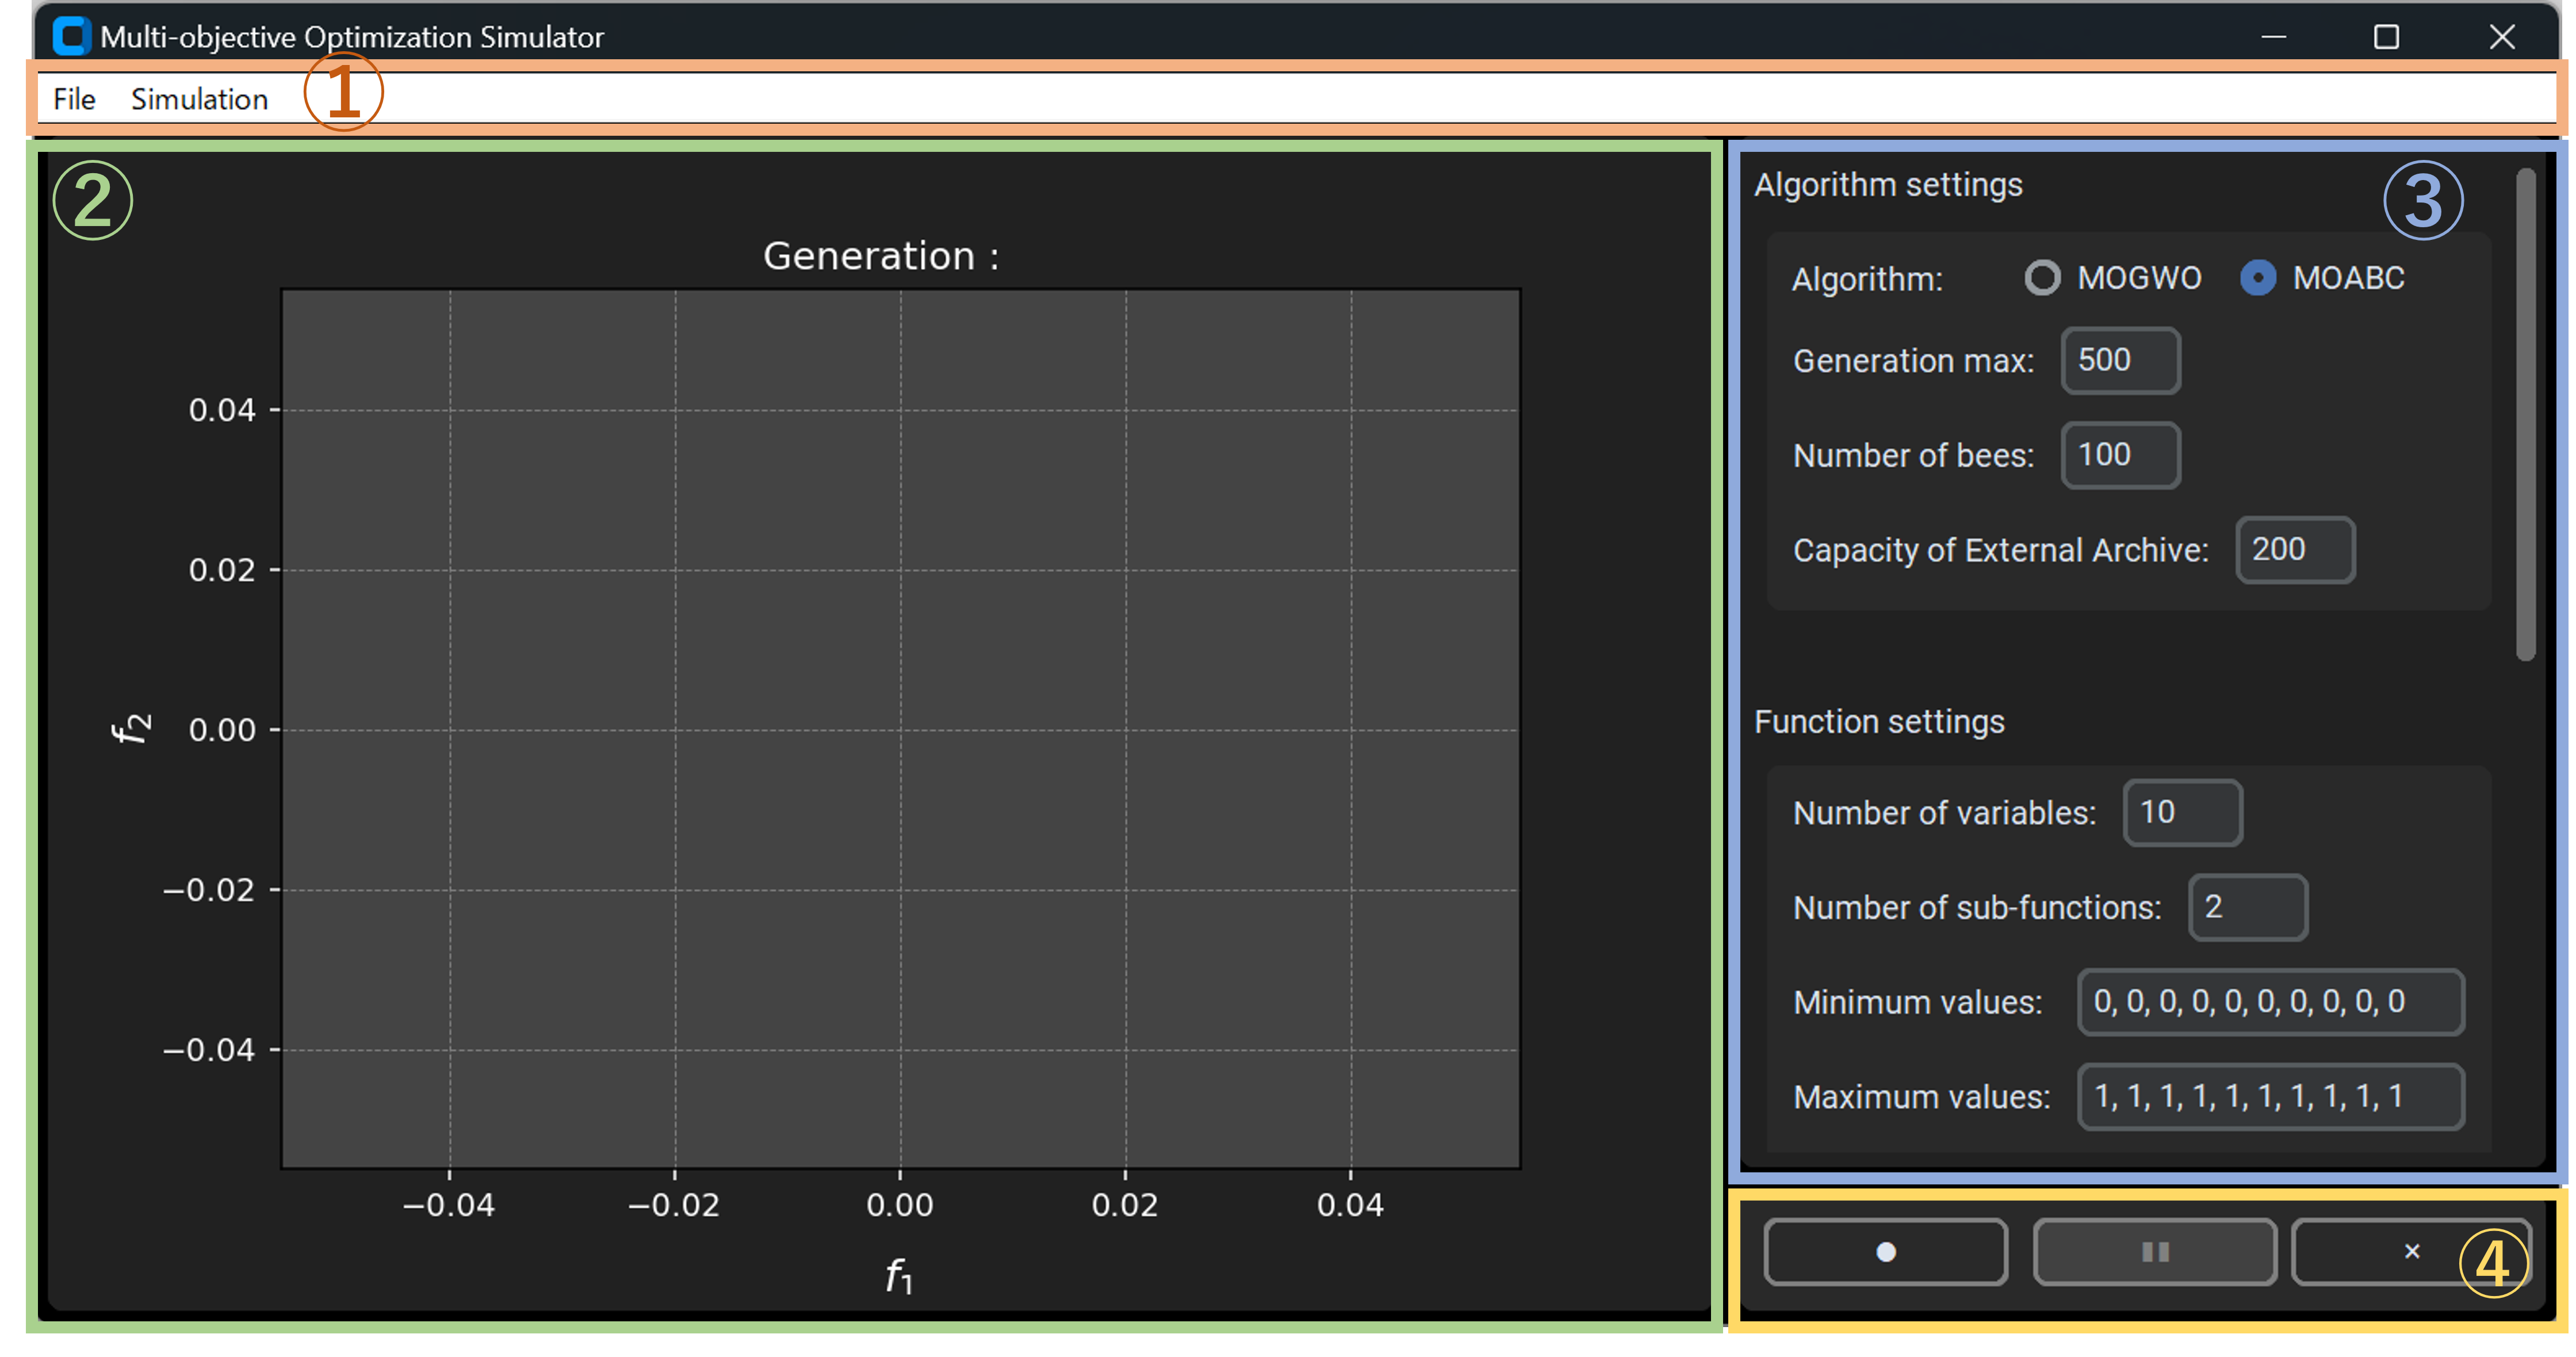
\includegraphics[width=\linewidth]{figures/window.png}
    \caption{シミュレーターの画面}
\end{figure}
図1は，シミュレータ―のウィンドウである．ウィンドウは，1.メニューバー，2.グラフ画面，3.設定画面，4.実行・停止ボタンの4つの部分から構成されている．以下では，これらの画面の見方と操作方法について説明する．
\subsection{メニューバー}
ウィンドウの上部にあるメニューバーには，「File」，「Simulation」2つのメニューがある．
\begin{itemize}
    \item \textbf{File}
        \begin{itemize}
            \item \textbf{Save Function Settings}\\
            入力されている関数とパレート最適解の設定をdat形式で保存する．
            \item \textbf{Load Function Settings}\\ 
            dat形式で保存された関数とパレート最適解の設定を読み込む．
            \item \textbf{Save Figure}\\
            グラフを保存する．グラフはpng形式またはpdf形式のどちらかを選択して保存することができる．
        \end{itemize}
    \item \textbf{Simulation}
        \begin{itemize}
            \item \textbf{Run Simulation}\\
            アルゴリズムを実行する．
            \item \textbf{Pose Simulation}\\
            アルゴリズムの実行を一時停止する．
        \end{itemize}
\end{itemize}
\subsection{グラフ}
ウィンドウ左側にあるグラフ画面には，アルゴリズムを実行して得られた外部アーカイブ内の非劣解の集合が表示される．横軸は目的関数1の値，縦軸は目的関数2の値であり，各非劣解は散布図としてプロットされる．また，パレート最適解の表示設定を有効にすればパレート最適解もグラフ上に点線で表示される．グラフ上部には，現在の反復回数が表示され，シミュレーションを一時停止すると被覆率（CR）も表示される．
\subsection{設定}
ウィンドウ右側にある設定画面でシミュレーションのパラメータや関数を設定することができる．主にアルゴリズムの設定（Algorithm settings），関数の設定（Function Settings）．パレート最適解の設定(True pareto front settings)の3つにわかれており，それぞれの設定を行うことでシミュレーションを実行できる．
\subsubsection{アルゴリズムのパラメータ設定}
\begin{itemize}
    \item \textbf{Algorithm}\\
        使用するアルゴリズムを選択する．MOABCまたはMOGWOを選択できる．
    \item  \textbf{Maximum Generation}\\
        最大世代数を整数値で設定する．世代数がこの値に達するとシミュレーションが終了する．
    \item \textbf{Population Size}\\
        Onlooker Bee や Gray Wolf の集団の個体数を整数値で設定する．
    \item \textbf{Capacity of External Archive}\\
        外部アーカイブの最大容量を整数値で設定する．外部アーカイブのサイズがこの値を超えると，混雑距離を用いて解を削除する．
\end{itemize}
\subsubsection{関数の設定}
ここでは，最適化する関数を設定する．このシミュレーターでは任意の数の変数を入力とした2つの目的関数 $f_1(\boldsymbol{x})$，$f_2(\boldsymbol{x})$ を設定することができる．
\begin{itemize}
    \item \textbf{Number of Variables}\\
        関数の変数の数を整数値で設定する．
    \item \textbf{Number of sub-functions}\\
        目的関数が複雑な形の場合，任意の個数のサブ関数 $g_i(\boldsymbol{x})$ を設定し，それらを組み合わせて目的関数を記述することができるようになっている．ここでは，サブ関数の個数を整数値で設定する．
    \item \textbf{Maximum Values}\\
        各変数の最大値を「,」区切りで入力する．
    \item \textbf{Minimum Values}\\
        各変数の最小値を「,」区切りで入力する．
    \item \textbf{g\_i}\\
        サブ関数 $g_i(\boldsymbol{x})$ を入力する．$g_i(\boldsymbol{x})$ は添え字が自分よりも小さいサブ関数 $g_j$ $(j < i)$ を用いて記述することができる．
    \item \textbf{f\_1，f\_2}\\
        目的関数 $f_1(\boldsymbol{x})$，$f_2(\boldsymbol{x})$ を入力する．$f_1(\boldsymbol{x})$，$f_2(\boldsymbol{x})$ はサブ関数 $g_i(\boldsymbol{x})$ を用いて記述することができる．
\end{itemize}
\textbf{数式の入力方法}\\
数式は，数式は基本的にPythonの構文に従って入力する．変数 $\boldsymbol{x} = (x_1, x_2, \cdots, x_n)$ は「x[1]」，「x[2]」，$\cdots$，「x[n]」として入力する．また，数式中には，Numpyに用いられる定数や関数を使用することができる．表1に数式中で使用可能な記号を示す．表1のNumpyの関数に加えて表2に示す関数も使用することができる．以下ではシミュレーターの入力例をいくつか示す．
\begin{table}[b]
    \centering
    \caption{数式中で使用できる記号}
    \begin{tabular}{ll|ll}
        \hline
        記号 & 説明 & 記号 & 説明  \\
        \hline
        pi & 円周率 & log2 & 底が2の対数\\
        e & ネイピア数 & sqrt & 平方根\\
        + & 加算 & power & 指数\\ 
        - & 減算 & arcsin & 逆正弦関数\\
        * & 乗算 & arccos & 逆余弦関数\\
        / & 除算 & arctan & 逆正接関数\\
        ** & べき乗 & sinh & 双曲線正弦関数\\
        // & 切り捨て除算 & cosh & 双曲線余弦関数\\
        abs & 絶対値 & tanh & 双曲線正接関数\\
        sin & 正弦関数& arcsinh & 双曲線逆正弦関数\\
        cos & 余弦関数 & arccosh & 双曲線逆余弦関数\\
        tan & 正接関数 & arctanh & 双曲線逆正接関数\\
        exp & 指数関数 & ceil & 天井関数\\
        log & 自然対数 & floor & 床関数\\
        log10 & 常用対数 & round & 四捨五入\\
        \hline
    \end{tabular}
\end{table}
\begin{table}[b]
    \centering
    \caption{その他の関数・記号}
    \begin{tabular}{ll} 
        \hline
        記号 & 説明 \\
        \hline
        N                       & 変数の数\\      
        if(条件, x, y)          & 条件が真のときx，偽のときy \\
        sum(a, b, h(x\_i))      & $\sum_{i=a}^{b}h(x_i)$ を計算する. 式中\\
                                & には,変数 $x_i$ を「x[i]」と記述\\
                                & できる \\
        product(a, b, h(x\_i))  & $\prod_{i=a}^{b}h(x_i)$ を計算する. 式中\\
                                & には,変数 $x_i$ を「x[i]」と記述\\
                                & できる \\
        \hline
    \end{tabular}
\end{table}
\newpage\noindent
\textbf{入力例1}\\
\quad 以下のような2目的最適化問題があるとする．
\begin{itembox}[l]{最適化問題1}
    \vspace{-15pt}
\begin{align*}
    \mbox{Mini} & \mbox{mize} \quad f_1, f_2\\
    \mbox{Subject}& \mbox{ to}  \\
                      & f_1 = x_1^2\\
                      & f_2 = (x_1-2)^2\\
                      & x_1 \in [-1000,1000]
\end{align*}
\end{itembox}
\quad このとき，シミュレーターには次のように入力することができる．
\begin{itembox}[l]{シミュレーターの入力}
    \vspace{-10pt}
\begin{lstlisting}[frame = none]
Number of Variables: 1
Number of sub-functions: 0
Minimum Values: -1e3
Maximum Values: 1e3
f_1: x[1]**2
f_2: (x[1]-2)**2
\end{lstlisting}
\end{itembox}

\noindent\textbf{入力例2}\\
\quad 今度は例1より複雑な目的関数を考えてみる．以下のような最適化問題が次で定義されているとする．
\begin{itembox}[l]{最適化問題2}
    \vspace{-15pt}
\begin{align*}
    \mbox{Mini} & \mbox{mize} \quad f_1, f_2\\
    \mbox{Subject}& \mbox{ to}  \\
                      & f_1 = x_1\\
                      & f_2 = g\times h\\
                      & g = 1+10\frac{\sum^N_{i = 2}x_i}{N-1}\\
                      & h = 1-\left(\frac{f_1}{g}\right)^{0.25}-\frac{f_1}{g}\sin(10\pi f_1)\\
                      & x_i \in [0,1], \quad (i = 1, \cdots, 10)
\end{align*}
\end{itembox}
\quad この問題は目的関数 $f_1$ と $f_2$ が別の関数 $g$，$h$ を使って定義されている．このような場合には，シミュレーター上にもサブ関数を用いて目的関数を記述することができる．このとき，関数の親子関係に注意する必要がある．問題では $h$ が $f1$ を用いて定義されているが，本シミュレーターはサブ関数が $f1$ を参照することができないため，少し書き換える必要がある．また，$h$ は $g$ を用いて定義されているため，サブ関数の入力時には $h$ が $g$ を参照できるように添え字に注意しなければならない．以上を考慮したうえで，シミュレーターには次のように入力することができる．

\begin{itembox}[l]{シミュレーターの入力}
    \vspace{-10pt}
\begin{lstlisting}[frame = none]
Number of Variables: 10
Number of sub-functions: 2
Minimum Values: 0,0,0,0,0,0,0,0,0,0
Maximum Values: 1,1,1,1,1,1,1,1,1,1
g_1: 1+10*sum(2,N,x[i])/(N-1)
g_2: 1-(x[1]/g[1])**0.25-(x[1]/g[1])*sin(10*pi*x[1])
f_1: x[1]
f_2: g[1]*g[2]
\end{lstlisting}
\end{itembox}

\subsubsection{パレート最適解の設定}
パレート最適解がわかっている場合，パレート最適解を設定してグラフ上に表示させることができる．目的関数の設定とは異なり，パレート最適解は1変数関数として入力する．パレート最適解の設定は以下のように行う．
\begin{itemize}
    \item \textbf{Show true pareto front}\\
        パレート最適解を表示するかどうかを設定する．
    \item \textbf{Minimum value}\\
        変数の最小値を入力する．
    \item \textbf{Maximum value}\\
        変数の最大値を入力する．
    \item \textbf{f\_1, f\_2}\\
        パレート最適解を入力する．目的関数と同様に，表1の数学記号を使用することができるが，1変数なので，sumやproductを使うことはできない．変数は「x[1]」として入力する．また，f[2]はf[1]を用いて記述することができる．
\end{itemize}
以下に入力例を示す．\\
\textbf{入力例}\\
最適化問題2のパレート最適解は $x_1 \in [0, 1]$，$x_i = 0$ $(i \neq 1)$ のときであり，次のように表せる．
\begin{itembox}[l]{最適化問題2のパレート最適解}
    \vspace{-20pt}
\begin{align*}
    &f_1: x_1\\
    &f_2: 1-x_1^{0.25}-x_1\sin(10\pi x_1)\\
    &x_1 \in [0, 1]
\end{align*}
\end{itembox}
これは次のようにしてシミュレーターに入力することができる．
\begin{itembox}[l]{シミュレーターの入力}
    \vspace{-10pt}
\begin{lstlisting}[frame = none]
Show true pareto front: True
Minimum Values: 0
Maximum Values: 1
f_1: x[1]
f_2: 1-x[1]**0.25-x[1]*sin(10*pi*x[1])
\end{lstlisting}
\end{itembox}


\subsection{実行・停止ボタン}
ウィンドウの右下には，3つのボタンがあり，それぞれ左から，シミュレーション開始ボタン，真ん中がシミュレーションの一時停止・再開ボタン，アプリケーションの終了ボタンになっている．3.3節で説明した設定を行った後，左側のボタンを押すことでシミュレーションを開始することができる．シミュレーションが開始されると，グラフ画面に非劣解の集合が表示され，アルゴリズムが実行される．シミュレーションを一時停止する場合は，中央のボタンを押すことで一時停止することができる．一時停止中に再開する場合は，再度中央のボタンを押すことで再開することができる．シミュレーターを使い終わったら，右側のボタンを押すことでアプリケーションを終了することができる．
\section{性能評価}
作成したシミュレーターを用いて各アルゴリズムの性能評価を行った．
\section{考察}
\end{document}
